\section{Программная реализация}
В данной главе рассмотрены уже существующие решения, связанные с генерацией отчетов, 
а также детально описана программная реализация полученной в рамках настоящей работы системы.

\subsection{Обзор существующих решений для генерации отчетов}
На данный момент существует множество систем, которые могут использоваться
для автоматической генерации отчетов по уже имеющимся данным: 
среди них есть, как простые, которые предоставляют интерфейс для построения
простых табличных отчетов на основе массива данных (например BandedReportGenerator\cite{BandedReportGenerator}),
так и более комплексные, предоставляющие возможность составления отчетов на основе 
языка RDL (Report Definition Language\cite{rdl_spec}), генерировать OLAP-кубы\cite{olap},
самостоятельно работать с подключением к источнику данных и т.д.

В рамках данного раздела рассмотрены два наиболее популярных программных комплекса
для работы с отчетами: ``SAP Crystal Reports''\cite{crystal_reports} и 
``SQL Server Reporting Services''\cite{sql_reporting} для Microsoft SQL Server, 
оценены их достоинства и недостатки, а также обосновано решение, принятое к реализации.

\subsubsection{SAP Crystal Reports}
\begin{figure}[!ht]
\begin{center}
\hspace*{-1cm} 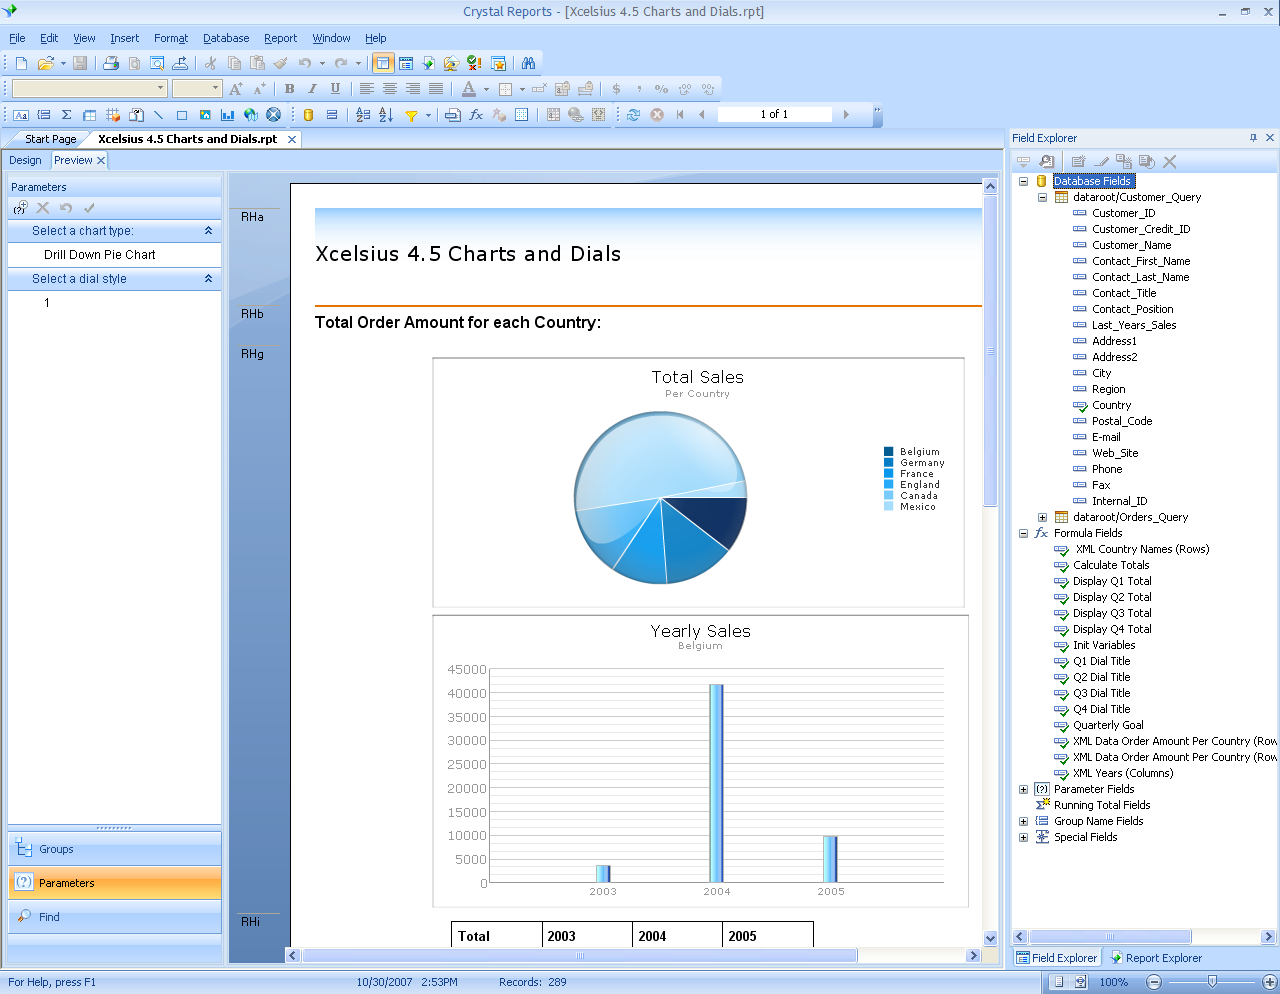
\includegraphics[scale=0.4]{../resources/CrystalReports2008.png}
\caption{Скриншот Crystal Reports 2008}
\label{gr:crystal_screenshot}
\end{center}
\end{figure}

\textit{Crystal Reports} является наиболее популярным продуктом компании SAP, состоит из
множества приложений таких как ``Crystal Reports Server'', ``Crystal Reports Viewer'',
``Crystal Reports Designer'', а так же плагина для Microsoft Visual Studio, позволяющего
составлять шаблоны отчетов в среде разработки.
 
\paragraph{Достоинства}
\begin{itemize}
\item{
Простой интерфейс для построения несложных отчетов.
}
\item{
Возможность генерации OLAP-кубов\cite{olap}, удобное представление
древообразной структуры отчета, описанной в \ref{section:stat_reports_task}.
}
\item{
Реализована работа с базой данных.
}
\item{
Реализована возможность графической интерпретации отчетов.
}
\end{itemize}

\paragraph{Недостатки}
\begin{itemize}
\item{
Отсутствие готовых решений для генерации отчетов через веб-интерфейс.
}
\item{
Недостаточная гибкость вычисления показателей, ограниченная пользовательскими формулами.
}
\item{
Инкапсуляция методов обработки данных, ограничивающая возможность оптимизировать
запросы к СУБД.
}
\end{itemize}

\subsubsection{SQL Server Reporting Services}
\begin{figure}[!ht]
\begin{center}
\hspace*{-1cm} 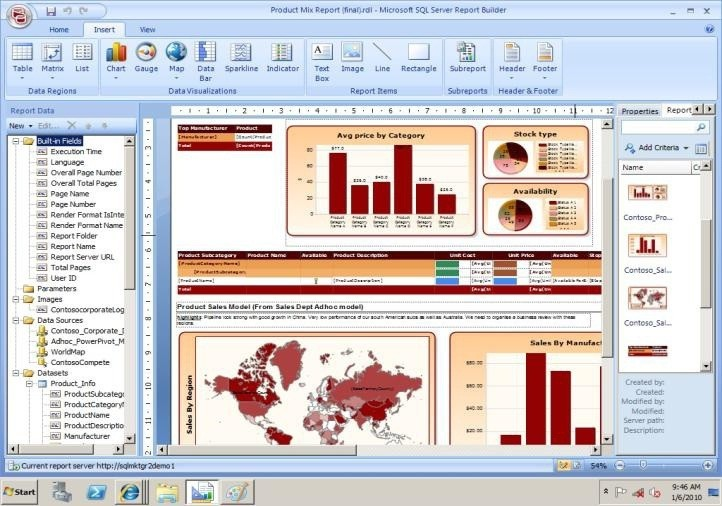
\includegraphics[scale=0.7]{../resources/SQLReporting.jpg}
\caption{Скриншот приложения Microsoft SQL Server Reporting Services 2008}
\label{gr:crystal_screenshot}
\end{center}
\end{figure}
Комплекс приложений \textit{SQL Server Reporting Services} создавался как конкурент для
\textit{SAP Crystal Reports}. В нем реализованы по сути те же базовые инструменты для конструирования
и просмотра отчетов, но при этом добавлены некоторые элементы функциональности, 
позволяющие Reporing Services занимать достойную позицию на рынке Business Intellegence технологий.

\paragraph{Достоинства}
\begin{itemize}
\item{
Более тесная интеграция с СУБД Microsoft SQL Server, которая в соответствии 
с нефункциональными требованиями к системе (см. \ref{part:requirements}) должна быть
использована в качестве хранилища данных.
}
\item{
Реализованы модули просмотра отчетов для ASP.NET\cite{sql_reporting}, что позволяет
реализовать генератор в виде веб-приложения.
}
\item{
Язык RDL\cite{rdl_spec}, реализованный на основе XML, позволяет специфицировать вид шаблона отчета,
на основе которого может быть сгенерирован отчет для пользователя, как через 
веб-интерфейс, так и с использованием Desktop-приложения.
}
\end{itemize}

\paragraph{Недостатки} В SQL Reporting Services присутствуют те же недостатки, что и в случае
с Crystal Reports, за исключением возможности генерации отчетов через веб-интерфейс.

\subsubsection{Результаты обзора}
Оба рассмотренные в предыдущих разделах программных продукта 
обладают неоспоримыми достоинствами, предлагая, как конечному пользователю, так и разработчику,
большой диапазон инструментов, позволяющих решать самый широкий круг задач.
Однако на первом этапе реализации системы было принято решение избежать их использования
в связи с серьезными рисками, возникающими в случае их применения в связи с
высокой степенью инкапсуляции механизмов построения отчетов в этих системах.

Возможные проблемы, вызванные инкапсуляцией включают:
\begin{itemize}
\item{
Невозможность достаточно тонкой настройки генератора может привести к несоответствиям в результате
работы генератора отчетов и требований к ним.
}
\item{
Невозможность оптимизации запросов к СУБД. Это может привести к тому, что при большом количестве данных
время генерации отчетов будет выходить за рамки, оговоренные в требованиях.
}
\end{itemize}

Таким образом в рамках данной работы было необходимо разработать оригинальный 
алгоритм генерации отчетов, результат работы которого должен удовлетворять требованиям,
описанным в первой главе.

При этом, учитывая факт использования в системе Microsoft SQL Server, не стоит исключать
возможность генерации более простых отчетов с помощью SQL Reporting Services, которое
пользователь сможеть осуществить самостоятельно при наличии доступа к серверу СУБД.



